% Network flow applications
Let $G = (V, E)$ a directed graph with source $s$ and sink $t$. Let $k > 0$.


\section{Decide whether there exists $k$ \textbf{edge}-disjoint paths}
We setup a network $N$ with source $s$ and sink $t$ based on graph $G$, setting the edges capacity and cost to 1. We then run a maxflow algorithm. Since edge capacity is 1, any edge used to transport one unit of flow from source to sink cannot be used in another path. Running any polynomial time maxflow algorithm then gives us a flow $F$. If $F \geq k$, then there exists at least $k$ edge-disjoint paths from $s$ to $u$ in $G$. Note that we can terminate the algorithm in constant time if $\text{outdegree}(s) < k$ or $\text{indegree(t)} < k$.

\section{Decide whether there exists $k$ \textbf{node}-disjoint paths}
We use a similar setup, with an additional trick allowing us to put constraints on the vertices rather than on the edges. In the network $N$, we represent each node $v \in V$ as two separate nodes $v_1$ and $v_2$, joint by an edge $e = (v_1, v_2)$. Inbound edges of $v$ are pointed to $v_1$, outbound edges leave from $v_2$.

Setting the capacity of $e$ to $+\infty$, this setup is equivalent to original graph. For this application, we set the capacity of $e$ to 1, ensuring that each node is used only once in the maxflow. All other capacities are set to $+\infty$ since we do not impose other constraints.

As before, running any polynomial time maxflow algorithm gives us a flow $F$, from which we deduce the result.

\section{Joining paths to form $k$ \textbf{edge}-disjoint paths}
% TODO

\section{Joining paths to form $k$ \textbf{node}-disjoint paths}
Suppose there exist $k$ node-disjoint paths from $s$ to $u \in V$, as well as $k$ node-disjoint paths from $u$ to $t$. We provide a counter-example with $k = 1$, showing that this does not imply there exists $k$ node-disjoint paths from $s$ to $t$.

\begin{figure}[ht]
  \center
  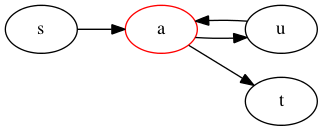
\includegraphics[width=2.5in]{figures/3-4-graph.png}
\end{figure}
